% Chapter 05 - Chemical Equilibrium.tex
% Copyright (c) 2014 - 2016, zhiayang@gmail.com
% Licensed under the Apache License Version 2.0.


\pagebreak
\part{Chemical Equilibrium}

	\section{Overview}

		Most of the reactions thus far have been irreversible, or uni-directional. However, many reactions in real life are actually in an
		equilibrium state --- at a certain stage, the rates of reaction for both the forward and backward reactions are equal, so the
		concentration of reactants and products do not change any further.

		The \itl{position of equilibrium} can be controlled to a certain extent, according to the principles of a man named
		\itl{Le Châtelier}. Lexically, an equilibrium reaction is represented with a double-hooked arrow, $⇋$, instead of a normal
		arrow, $→$.

		\subsection{Dynamic Equilibrium}

			It is important to note that this state of equilibrium is a \itl{dynamic} equilibrium; the rate of the forward and backward
			reactions are \itl{equal} and \itl{non-zero}. If both the rates of reaction are zero, then it is in a state of \itl{static}
			equilibrium. Unless the reaction mixture is disturbed, the system will remain in this equilibrium.

			The nature of equilibrium reactions means that they can be \enquote{started} from either direction, beginning with only reactants or
			only products. The system will eventually move back into the position of equilibrium.

		% end subsection

		\pagebreak
		\subsection{Graphs}

			\subsubsection{Concentration-Time}

				\graphdiagram[1.0]{
					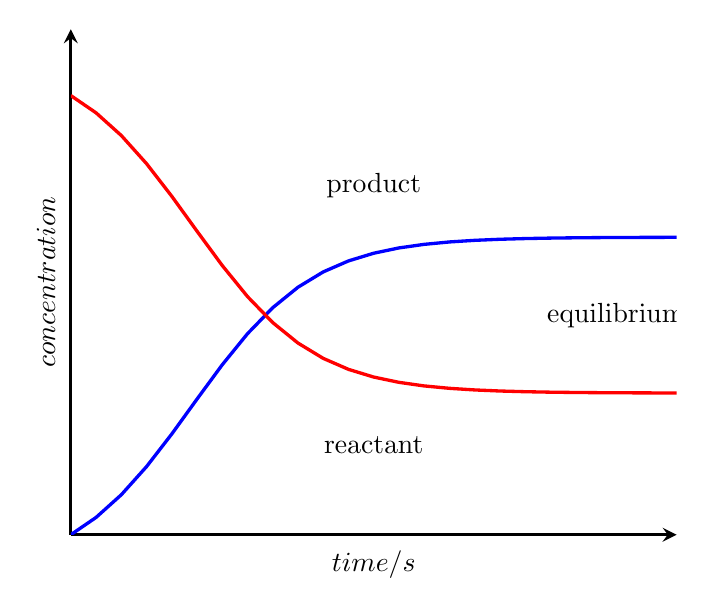
\begin{tikzpicture}

						\begin{axis}[
							axis lines		= left,
							domain			= 0.5:3,
							xlabel			= \textbf{$time/s$},
							ylabel			= \textbf{$concentration$},
							axis line style	= very thick,
							height			= 80mm,
							ytick			= \empty,
							xtick			= \empty,
						]

							\addplot[color = blue, very thick, restrict x to domain = 0.5:3]{
								0.65 * (1 / (1 + e^(-(4*x - 4))))
							};

							\addplot[color = red, very thick, restrict x to domain = 0.5:3]{
								1 - 0.65 * (1 / (1 + e^(-(4*x - 4))))
							};

							\addplot[color = green, opacity = 0.0, very thick]{
								1.05
							};

							\node at (axis cs: 1.75, 0.25) {reactant};
							\node at (axis cs: 1.75, 0.75) {product};
							\node at (axis cs: 2.75, 0.5) {equilibrium};

						\end{axis}
					\end{tikzpicture}

				}[Both gradients reach 0 at the equilibrium]

			% end subsubsection


			\subsubsection{Rate-Time}

				\graphdiagram[1.0]{
					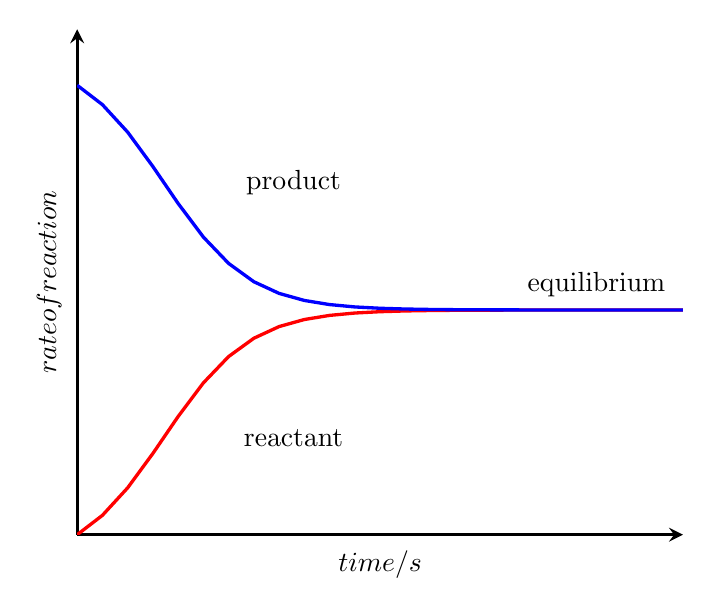
\begin{tikzpicture}

						\begin{axis}[
							axis lines		= left,
							domain			= 0.5:4,
							xlabel			= \textbf{$time/s$},
							ylabel			= \textbf{$rate of reaction$},
							axis line style	= very thick,
							height			= 80mm,
							ytick			= \empty,
							xtick			= \empty,
						]

							\addplot[color = red, very thick, restrict x to domain = 0.5:4]{
								0.5 * (1 / (1 + e^(-(4*x - 4))))
							};

							\addplot[color = blue, very thick, restrict x to domain = 0.5:4]{
								1 - 0.5 * (1 / (1 + e^(-(4*x - 4))))
							};

							\addplot[color = green, opacity = 0.0, very thick]{
								1.05
							};

							\node at (axis cs: 1.75, 0.25) {reactant};
							\node at (axis cs: 1.75, 0.75) {product};
							\node at (axis cs: 3.5, 0.55) {equilibrium};

						\end{axis}
					\end{tikzpicture}

				}[The rates of reaction meet in the centre and are equal at the position of equilibrium.]

			% end subsubsection

		% end subsection

		\pagebreak
		\subsection{Position of Equilibrium}

			From the concentration-time graph, it is possible to determine if the position of equilibrium lies more to the \itl{left} or the
			\itl{right}. The former means that the the forward reaction is favoured more (reading equations from left-to-right), while the
			latter indicates a more favoured backwards reaction.

			\graphdiagram[1.0]{
				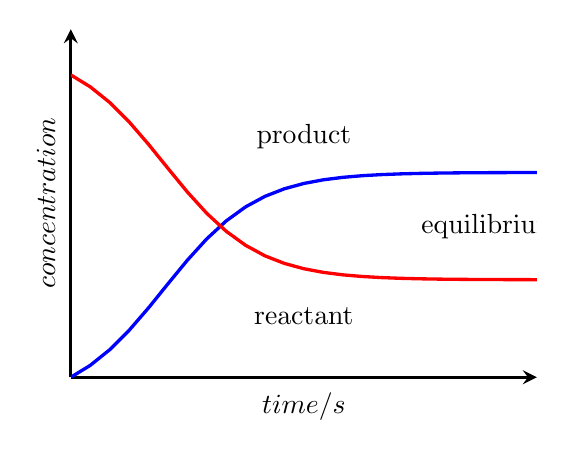
\begin{tikzpicture}

					\begin{axis}[
						axis lines		= left,
						domain			= 0.5:3,
						xlabel			= \textbf{$time/s$},
						ylabel			= \textbf{$concentration$},
						axis line style	= very thick,
						height			= 60mm,
						width			= 75mm,
						ytick			= \empty,
						xtick			= \empty,
					]

						\addplot[color = blue, very thick, restrict x to domain = 0.5:3]{
							0.65 * (1 / (1 + e^(-(4*x - 4))))
						};

						\addplot[color = red, very thick, restrict x to domain = 0.5:3]{
							1 - 0.65 * (1 / (1 + e^(-(4*x - 4))))
						};

						\addplot[color = green, opacity = 0.0, very thick]{
							1.05
						};

						\node at (axis cs: 1.75, 0.25) {reactant};
						\node at (axis cs: 1.75, 0.75) {product};
						\node at (axis cs: 2.75, 0.5) {equilibrium};

					\end{axis}
				\end{tikzpicture}
				\hspace{10mm}
				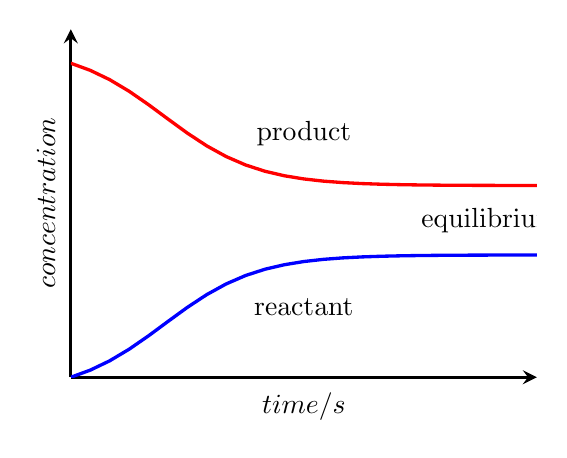
\begin{tikzpicture}

					\begin{axis}[
						axis lines		= left,
						domain			= 0.5:3,
						xlabel			= \textbf{$time/s$},
						ylabel			= \textbf{$concentration$},
						axis line style	= very thick,
						height			= 60mm,
						width			= 75mm,
						ytick			= \empty,
						xtick			= \empty,
					]

						\addplot[color = blue, very thick, restrict x to domain = 0.5:3]{
							0.40 * (1 / (1 + e^(-(4*x - 4))))
						};

						\addplot[color = red, very thick, restrict x to domain = 0.5:3]{
							1 - 0.40 * (1 / (1 + e^(-(4*x - 4))))
						};

						\addplot[color = green, opacity = 0.0, very thick]{
							1.05
						};

						\node at (axis cs: 1.75, 0.25) {reactant};
						\node at (axis cs: 1.75, 0.75) {product};
						\node at (axis cs: 2.75, 0.5) {equilibrium};

					\end{axis}

				\end{tikzpicture}
			}

			In the system on the left, the final concentration of products is greater than the final concentration of reactants;
			\itl{ie.} the position of equilibrium is further to the right. Conversely, the position of equilibrium is to the left
			in the graph on the right.


		% end subsection

	% end section


	\pagebreak
	\section{Equilibrium Constants}

		There are two equilibrium constants, \Kc{} and \Kp{}, that serve roughly the same purpose in different contexts --- the former for normal,
		aqueous reactions where normal concentrations apply, and the latter for gaseous systems where it is more logical to use partial pressures.

		\subsection{Equilibrium Constant \texorpdfstring{\MKc{}}{Kc}}

			\Kc{} is calculated using the concentrations of each product and each reactant, \itl{at equilibrium}. For the reaction below:

			\txtdiagram{
				\schemestart[0,1.0,thick]
					\ch{p}\hspace{0.1em}\ch{A}\hspace{2mm} + \hspace{2mm}\ch{q}\hspace{0.1em}\ch{B}
					\arrow
					\ch{r}\hspace{0.1em}\ch{C}\hspace{2mm} + \hspace{2mm}\ch{s}\hspace{0.1em}\ch{D}
				\schemestop
			}{}

			The corresponding \Kc{} would be as such:

			\txtdiagram{
				\[K_{c} = \frac{[C]^{c}[D]^{d}}{[A]^{a}[B]^{b}}\]
			}{}

			Note that it is \itl{products over reactants}. The power that each concentration is raised to is simply the stoichiometric
			coefficient of that reactant or product, nothing more --- far simpler than the rate equation nonsense.

			The reason is that

		% end subsection


		\subsection{Gaseous Equilibrium Constant \texorpdfstring{\MKp{}}{Kp}}

			In situations where it is more convenient to use partial pressures, then it is as simple as substituting the concentrations
			in the original \Kc{} equation with the corresponding partial pressures to get \Kp{}, like so:

			\txtdiagram{
				\[K_{p} = \frac{(P_{C})^{c}(P_{D})^{d}}{(P_{A})^{a}(P_{B})^{b}}\]
			}{}

			This works because the partial pressure is simply a equivalent to the mole ratio of the particular gas to the total number of
			moles of gas in the system -- when put together, the total moles cancel, leaving what is effectively the stoichiometric
			coefficient.

		% end subsubsection


		\pagebreak
		\subsection{Determination of Position of Equilibrium}

			From the equations of \Kc{} and \Kp{} above, it can be seen that when the numerator and denominator are equal, then the values of
			\Kc{} and \Kp{} become $1$. At this point, the position of equilibrium lies perfectly in the centre, favouring neither the forward
			nor backward reactions.

			Applying the knowledge of fractions, the larger the value of \Kc{}, then the further forward lies the position of equilibrium.
			Conversely, the smaller the value, the further backward it lies.

			\graphdiagram[1.0]{
				\begin{tikzpicture}
					\begin{axis}[
						y				= 1.5cm,	% y unit vector
						hide y axis,				% hide the y axis
						axis x line*	= bottom,	% only show the bottom x axis line, without an arrow tip
						xmin			= 0,
						xmax			= 10,		% range for the x axis
						xlabel			= \Kc{} or \Kp{},
						width			= 160mm,
						xtick			= {0.0, 4, 5, 6, 10},
						xticklabels		= {0, 10\sps{-3}, 1, 10\sps{3}, ∞},
					]

					\addplot [no markers, very thick, green, opacity = 0.0] table[col sep=comma, row sep=crcr] {
						0, 1    \\
						10, 1   \\
					};

					\node at (axis cs: 3, 1.2) {left};
					\node at (axis cs: 7, 1.2) {right};

					\end{axis}
				\end{tikzpicture}
			}

			\Kc{} values around \num{1e-3} to \num{1e3} are considered systems where the position of equilibrium is relatively centred,
			while values outside of that range indicate a system strongly preferring either the forward or reverse reaction.

		% end subsection


		\subsection{Equilibrium Quotients \texorpdfstring{\itl{Q\sbs{c}}}{Qc} and \texorpdfstring{\itl{Q\sbs{p}}}{Qp}}

			\Qc{} and \Qp{} are essentially exactly the same as \Kc{} and \Kp{}, except the $Q$ values represent the position of equilibrium
			\itl{at that instant}. Thus, it is often useful to compare the \Qc{} and \Kc{} values for a system, to determine
			where the \itl{current} position of equilibrium lies, and which direction the system is currently proceeding in.

			There are 3 cases, as there always are when comparing two numbers:

			\begin{bulletlist}
				& $Q < K$; the current position is too far left, and the system proceeds in the \itl{forward} direction until equilibrium
				is achieved

				& $Q = K$; the system is currently at equilibrium, and will remain so unless disturbed

				& $Q > K$; the current position is too far left, and the system proceeds in the \itl{reverse} direction until equilibrium
				is achieved.
			\end{bulletlist}

			Naturally, the value of $Q$ uses the same formula, except with the \itl{instantaneous} values for concentration or partial
			pressure.

		% subsection

	% end section



	\pagebreak
	\section{Factors Affecting Equilibrium Position}

		\subsection{Le Châtelier's Principle}

			This man's principle governs exactly how various changes to a system at equilibrium will result in a shift in the position of
			said equilibrium.

			\itl{When any system at equilibrium is subjected to change in concentration, temperature, volume, or pressure, then the
			system readjusts itself to (partially) counteract the effect of the applied change and a new equilibrium is established.}

			--- \itl{Henry Louis Le Châtelier}

			In short, the system will attempt to compensate for, and reverse, any changes made to it by an external agent, through a shift
			in the position of equilibrium.

		% end subsection


		\subsection{Changes in Concentration or Partial Pressure}

			This is the most direct method to affect the system. If the concentration of one or more reactants is increased, then the
			concentration difference deviates from the equilibrium. Thus, the system will attempt to compensate by shifting \itl{forwards},
			in an attempt to consume the reactant and bring the concentration ratio back to an acceptable range.

			The idea above applies in reverse when increasing the concentration of one or more products, and indeed applies for gaseous
			systems using partial pressures as well.

		% end subsection



		\subsection{Changes in Total (System) Pressure}

			Unlike a change in the partial pressure of a reactant or product, changing the total pressure of the system affects both
			the products and reactants.

			Using the reaction for the formation of ammonia, \ch{NH3}, from \ch{H2} and \ch{N2}:

			\txtdiagram{
				\schemestart[0,1.0,thick]
					\ch{N2 \stG}\hspace{2mm} + \hspace{2mm}\ch{3 H2 \stG}
					\arrow{<=>}
					\ch{2 NH3 \stG}
				\schemestop
			}{}

			The forward reaction changes the number of moles of gas from \num{4} (\num{1} + \num{3}) to \num{2}, resulting in a net
			\itl{decrease}; the backwards reaction would thus increase the number of moles of gas from \num{2} to \num{4}, a net
			\itl{increase}.

			When the total pressure is \itl{increased}, the system will attempt to reduce it, by reducing the number of moles of gas
			in the system --- thus moving the position of equilibrium \itl{to the right}, favouring the production of \ch{NH3}.

			\pagebreak
			If the total number of moles of gas on either side of the reaction are the same, for example:

			\txtdiagram{
				\schemestart[0,1.0,thick]
					\ch{H2 \stG}\hspace{2mm} + \hspace{2mm}\ch{Br2 \stG}
					\arrow{<=>}
					\ch{2 HBr \stG}
				\schemestop
			}{}

			Then a change in the pressure of the system will have \itl{no effect} on the position of equilibrium.

		% end subsection


		\subsection{Changes in Temperature}

			Changes in temperature will shift the equilibrium in an attempt to reduce the change --- in this case, the enthalpy change
			of the reaction is used, since it determines whether the reaction will result in a net release or absorption of heat.

			Again, using the formation of ammonia:

			\txtdiagram{
				\schemestart[0,1.0,thick]
					\ch{N2 \stG}\hspace{2mm} + \hspace{2mm}\ch{3 H2 \stG}
					\arrow{<=>}
					\ch{2 NH3 \stG}
				\schemestop
			}{\enth{} = \SI{-92.4}{\kilo\joule\per\mole}}

			The forward reaction is \itl{exothermic} as given by the negative \enth{}. Thus, a \itl{decrease} in temperature will
			make the system attempt to compensate by increasing the temperature. Since the forward reaction \itl{releases heat}, it will
			be favoured, and the position of equilibrium moves to the \itl{right}.

			Naturally, the reverse applies.

		% end subsection


		\subsection{Presence of Catalyst}

			This section is a red herring --- adding or removing a catalyst \itl{does not} change the position of equilibrium, since the
			rate of reaction for \itl{both} the forward and backward reactions are increased or decreased by an equal amount.

			Thus, catalysts only change the amount of time taken to \itl{reach} equilibrium, not its position.

		% end subsection

	% end section


	\pagebreak
	\section{The Process of Haber}

		\subsection{Overview}

			The \itl{Haber Process} is an important, industrially-used process for the manufacture of ammonia (\ch{NH3}), which is widely
			used for fertiliser.

			\itl{My name is Fritz Haber, and I maked a process. It was all me, Carl Bosch did nothing.}

			--- \itl{Fritz Haber}

			As shown above, the formation of \ch{NH3} from \ch{H2} and \ch{N2} is an equilibrium, and unfortunately the position of equilibrium
			likes quite far to the left --- hence the need for expensive industrial equipment to produce this at scale.


			\txtdiagram{
				\schemestart[0,1.0,thick]
					\ch{N2 \stG}\hspace{2mm} + \hspace{2mm}\ch{3 H2 \stG}
					\arrow{<=>}
					\ch{2 NH3 \stG}
				\schemestop
			}{}


			To increase the yield of ammonia, 3 techniques are used:


			\begin{bulletlist}
				& The pressures of \ch{H2} and \ch{N2} are kept as high as practically possible
				& \ch{NH3} formed is removed as soon as possible, to reduce its concentration
				& The rate of reaction is increased using iron powder.
			\end{bulletlist}

			A note on the last point --- while it does not move the position of equilibrium and speeds up both reactions, if the
			position of equilibrium is already to the right, there will be a net gain.

		% end subsection


		\pagebreak
		\subsection{Process}

			\imgdiagram{140mm}{../figures/physical/ch05/haber_process.png}{\vspace{-2em}}

			The image should be fairly self-explanatory. Pure nitrogen gas is obtained from liquefied air, while hydrogen gas is obtained
			via methane (\ch{CH4}) and steam in the presence of a catalyst.

			\subsubsection{Conditions}

				In a rare occasion for this series, some figures must be memorised. Note that while Le Châtelier's Principle would imply
				low temperatures, the temperature is typically kept (relatively) high to allow for the reaction to proceed at an appreciable
				rate. It's one thing for the position of equilibrium to be far forward, it's another thing for the forward reaction to
				actually occur.

				\vspace{1.5em}
				\vbox{\textbf{Conditions:}\tabto{35mm}\SI{450}{\celsius}, \SI{250}{\atm}, Finely divided \ch{Fe} catalyst.}

			% end subsubsection

		% end subsection

	% end section

% end part
















